%%%%%%%%%%%%%%%%%%%%%%%%%%%%%%%%%%%%%%%
% Wenneker Resume/CV
% LaTeX Template
% Version 1.1 (19/6/2016)
%
% This template has been downloaded from:
% http://www.LaTeXTemplates.com
%
% Original author:
% Frits Wenneker (http://www.howtotex.com) with extensive modifications by 
% Vel (vel@LaTeXTemplates.com)
%
% License:
% CC BY-NC-SA 3.0 (http://creativecommons.org/licenses/by-nc-sa/3.0/
%
%%%%%%%%%%%%%%%%%%%%%%%%%%%%%%%%%%%%%%

%----------------------------------------------------------------------------------------
%	PACKAGES AND OTHER DOCUMENT CONFIGURATIONS
%----------------------------------------------------------------------------------------

\documentclass[a4paper,12pt]{memoir} % Font and paper size

%%%%%%%%%%%%%%%%%%%%%%%%%%%%%%%%%%%%%%%%%
% Wenneker Resume/CV
% Structure Specification File
% Version 1.1 (19/6/2016)
%
% This file has been downloaded from:
% http://www.LaTeXTemplates.com
%
% Original author:
% Frits Wenneker (http://www.howtotex.com) with extensive modifications by 
% Vel (vel@latextemplates.com)
%
% License:
% CC BY-NC-SA 3.0 (http://creativecommons.org/licenses/by-nc-sa/3.0/)
%
%%%%%%%%%%%%%%%%%%%%%%%%%%%%%%%%%%%%%%%%%

%----------------------------------------------------------------------------------------
%	PACKAGES AND OTHER DOCUMENT CONFIGURATIONS
%----------------------------------------------------------------------------------------

\usepackage{XCharter} % Use the Bitstream Charter font
\usepackage[utf8]{inputenc} % Required for inputting international characters
\usepackage[T1]{fontenc} % Output font encoding for international characters

\usepackage[top=1cm,left=1cm,right=1cm,bottom=1cm]{geometry} % Modify margins

\usepackage{graphicx} % Required for figures

\usepackage{flowfram} % Required for the multi-column layout

\usepackage{url} % URLs
\usepackage{hyperref}

\hypersetup{
    colorlinks=true,
    linkcolor=cyan,
    filecolor=magenta,      
    urlcolor=RoyalBlue,
}

\usepackage[usenames,dvipsnames]{xcolor} % Required for custom colours

\usepackage{tikz} % Required for the horizontal rule

\usepackage{enumitem} % Required for modifying lists
\setlist{noitemsep,nolistsep} % Remove spacing within and around lists

\setlength{\columnsep}{\baselineskip} % Set the spacing between columns

% Define the left frame (sidebar)
\newflowframe{0.22\textwidth}{\textheight}{0pt}{0pt}[left]
\newlength{\LeftMainSep}
\setlength{\LeftMainSep}{0.22\textwidth}
\addtolength{\LeftMainSep}{1\columnsep}
 
% Small static frame for the vertical line
\newstaticframe{1.5pt}{\textheight}{\LeftMainSep}{0pt}
 
% Content of the static frame with the vertical line
\begin{staticcontents}{1}
\hfill
\tikz{\draw[loosely dotted,color=RoyalBlue,line width=1.5pt,yshift=0](0,0) -- (0,\textheight);}
\hfill\mbox{}
\end{staticcontents}
 
% Define the right frame (main body)
\addtolength{\LeftMainSep}{1.5pt}
\addtolength{\LeftMainSep}{1\columnsep}
\newflowframe{0.7\textwidth}{\textheight}{\LeftMainSep}{0pt}[main01]

\pagestyle{empty} % Disable all page numbering

\setlength{\parindent}{0pt} % Stop paragraph indentation

%----------------------------------------------------------------------------------------
%	NEW COMMANDS
%----------------------------------------------------------------------------------------

\newcommand{\userinformation}[1]{\renewcommand{\userinformation}{#1}} % Define a new command for the CV user's information that goes into the left column

\newcommand{\cvheading}[1]{{\Huge\bfseries\color{RoyalBlue} #1} \par\vspace{.6\baselineskip}} % New command for the CV heading
\newcommand{\cvsubheading}[1]{{\Large\bfseries #1} \bigbreak} % New command for the CV subheading

\newcommand{\Sep}{\vspace{1em}} % New command for the spacing between headings
\newcommand{\SmallSep}{\vspace{0.5em}} % New command for the spacing within headings

\newcommand{\aboutme}[2]{ % New command for the about me section
\textbf{\color{RoyalBlue} #1}~~#2\par\Sep
}
	
\newcommand{\CVSection}[1]{ % New command for the headings within sections
{\Large\textbf{#1}}\par
\SmallSep % Used for spacing
}

\newcommand{\CVItem}[2]{ % New command for the item descriptions
\textbf{\color{RoyalBlue} #1}\par
#2
\SmallSep % Used for spacing
}

\newcommand{\bluebullet}{\textcolor{RoyalBlue}{$\circ$}~~} % New command for the blue bullets
 % Include the file specifying document layout and packages

%----------------------------------------------------------------------------------------
%	NAME AND CONTACT INFORMATION 
%----------------------------------------------------------------------------------------

\userinformation{ % Set the content that goes into the sidebar of each page
\begin{flushright}
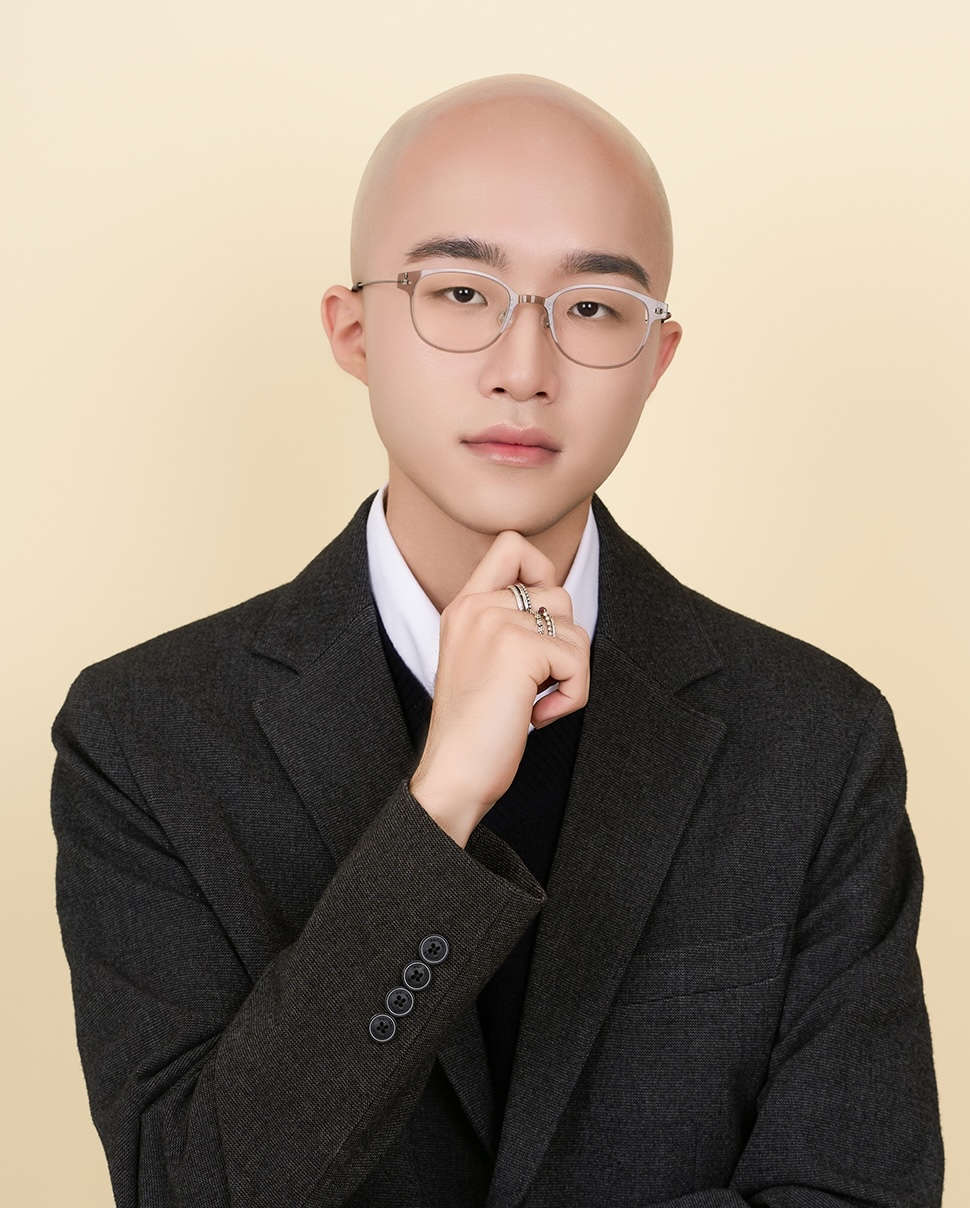
\includegraphics[width=0.8\columnwidth]{profile_photo.jpg}\\[\baselineskip] % Your photo
\Large
Jaewoo Jung \\ % Your name
\hypersetup{urlcolor=cyan}
\small
\href{mailto:lukael.jung@gmail.com}{\nolinkurl{lukael.jung@gmail.com}} \\ % Your email address
\url{https://lukael.kr} \\ % Your URL
(+82)10-3063-7584 \\ % Your phone number
\Sep % Some whitespace
\textbf{Address} \\
Seoul,
Republic of Korea \\ % Address 3
\vfill % Whitespace under this block to push it up under the photo
\end{flushright}
}

%----------------------------------------------------------------------------------------

\begin{document}

\userinformation % Print your information in the left column

\framebreak % End of the first column

%----------------------------------------------------------------------------------------
%	HEADING
%----------------------------------------------------------------------------------------

\cvheading{Jaewoo Jung} % Large heading - your name

\cvsubheading{University Student} % Subheading - your occupation/specialization

% %----------------------------------------------------------------------------------------
% %	ABOUT ME
% %----------------------------------------------------------------------------------------

% \aboutme{About Me}
% {}

%----------------------------------------------------------------------------------------
%	EDUCATION
%----------------------------------------------------------------------------------------

\CVSection{Education}

%------------------------------------------------

\CVItem{2013 - 2015, Changwon Science High School}{Chemistry}

%------------------------------------------------

\CVItem{2015 - present, Yonsei University}{Electrical and Electronic Engineering}

%------------------------------------------------

\Sep % Extra whitespace after the end of a major section

%----------------------------------------------------------------------------------------
%	EXPERIENCE
%----------------------------------------------------------------------------------------

\CVSection{Experience}

%------------------------------------------------

\CVItem{Mar 2017 - Dec 2017, \textit{Research Engineer}, Luxrobo}{
Detailed achievements:
\begin{itemize}
	\item Network Module Firmware
	\begin{itemize}
		\item C/C++
		\item FreeRTOS
		\item Wi-Fi
		\item BLE
		\item USART
	\end{itemize}

	\item OS Development
	\begin{itemize}
		\item RTOS research
		\item Contiki OS
	\end{itemize}

	\item Bluetooth 5
	\begin{itemize}
		\item Nordic nRF52DK
		\item Mesh Network
	\end{itemize}

	\item NLP
	\begin{itemize}
		\item Chatscript
		\item Slack-Chatscript Linkage(Python)
	\end{itemize}

\end{itemize}
}

%------------------------------------------------

%------------------------------------------------

\CVItem{Dec 2016 - Mar 2017, \textit{Internship}, Yonsei Biocybernetics Lab}{
Detailed achievements:
\begin{itemize}
	\item Swarm robotics
	\begin{itemize}
		\item Hardware
		\begin{itemize}
			\item FreeRTOS
			\item Wi-Fi
			\item Bluetooth
			\item Vibration Control
		\end{itemize}
		\item Software
		\begin{itemize}
			\item openCV
			\item Formation
			\item Shepharding
			\item Task Allocation
		\end{itemize}
	\end{itemize}
\end{itemize}
}

%------------------------------------------------

\CVItem{Jan 2017 - Dec 2017, \textit{President}, SBTM}
{Robot club in Yonsei University}

%------------------------------------------------

\Sep % Extra whitespace after the end of a major section

%----------------------------------------------------------------------------------------
%	NEW PAGE DELIMITER
%	Place this block wherever you would like the content of your CV to go onto the next page
%----------------------------------------------------------------------------------------

\clearpage % Start a new page

\userinformation % Print your information in the left column

\framebreak % End of the first column

%----------------------------------------------------------------------------------------
%	SKILLS
%----------------------------------------------------------------------------------------

\CVSection{Software Development Skills}

%------------------------------------------------

\CVItem{Programming}
{\begin{tabular}{p{0.2\textwidth} p{0.2\textwidth} p{0.2\textwidth}}
\bluebullet C/C++ &  \bluebullet Python & \bluebullet Matlab\\
% \bluebullet C/C++ &  \bluebullet PHP & \bluebullet Matlab\\
\end{tabular}}

%------------------------------------------------

\CVItem{Computer Software}
{\begin{tabular}{p{0.2\textwidth} p{0.2\textwidth} p{0.2\textwidth}}
\bluebullet Unity(C\#) &  \bluebullet Eagle CAD & \bluebullet Inventor\\
\end{tabular}}

%------------------------------------------------

\Sep % Extra whitespace after the end of a major section

%----------------------------------------------------------------------------------------
%	Competitions
%----------------------------------------------------------------------------------------

\CVSection{Competitions}

%------------------------------------------------

\CVItem{2013, \href{https://www.gnse.kr/bbs.php?id=gnse32&num=2}{\textit{Student Science Invention Competition}}, GNSE}
{\textit{Easy Bookbinding Tape Cutter}}

%------------------------------------------------

%------------------------------------------------

\CVItem{2013, \textit{Student Creativity Festival}, GNE}
{\textit{Between Ventilation and Insulation}}

%------------------------------------------------

%------------------------------------------------

\CVItem{2013, \href{http://www.eswcontest.com}{\textit{Embedded Software Contest}}, KESSIA}
{\textit{Minesweeper Robot using LEGO Mindstorm}\\{Hardware Engineer}}

%------------------------------------------------

%------------------------------------------------

\CVItem{2013, \textit{R\&E Festival}, KOSAF}
{\textit{Develop Filters made from ESM's Toxic substances Absorptive Ability}}

%------------------------------------------------

%------------------------------------------------

\CVItem{2014, \href{https://www.gnse.kr/bbs.php?id=gnse32&num=2}{\textit{Student Science Invention Competition}}, GNSE}
{\textit{Mono/Stereo Earphone}}

%------------------------------------------------

%------------------------------------------------

\CVItem{2014, \textit{ISEF-K}, KOFAC}
{\textit{Study on Gas phase Adsorption of Toxic substances on ES, ESM and Filter}}

%------------------------------------------------

%------------------------------------------------

\CVItem{2014, \href{https://www.gnse.kr/bbs.php?id=gnse31&num=1}{\textit{Science Exhibition}}, GNSE}
{\textit{Measuring Chemical reaction rate using Smartphone}}

%------------------------------------------------

%------------------------------------------------

\CVItem{2014, \textit{Steam R\&E Festival}, KOFAC}
{\textit{Smartphone Application for Chemistry Experiment}}

%------------------------------------------------

%------------------------------------------------

\CVItem{2016, \href{http://race.acelab.org/}{\textit{Smart Model Car Competition}}, Hanyang University}
{\textit{Autonomous driving Model Car}\\{Hardware Team}}

%------------------------------------------------

%------------------------------------------------

\CVItem{2016, \href{http://www.koreauav.com/}{\textit{Korea Robot Aircraft Competition}}, KAIA}
{\textit{Autonomous driving Quadcopter}\\{Team Leader, Hardware Engineer}}

%------------------------------------------------

%------------------------------------------------

\CVItem{2017, \href{http://race.acelab.org/}{\textit{Smart Model Car Competition}}, Hanyang University}
{\textit{Autonomous driving Model Car}\\{Team Leader, Hardware Engineer}}

%------------------------------------------------

%------------------------------------------------

\CVItem{2018, \href{http://mgreencar.co.kr/}{\textit{International Student Car Competition}}, KTSA}
{\textit{Autonomous driving Cart}\\{LIDAR Team}}

%------------------------------------------------

\Sep % Extra whitespace after the end of a major section

\clearpage % Start a new page

\userinformation % Print your information in the left column

\framebreak % End of the first column

%----------------------------------------------------------------------------------------
%	AWARDS
%----------------------------------------------------------------------------------------

% \CVSection{Awards}

% %------------------------------------------------

% \CVItem{2013, \textit{Silver Awards}, Cornell University}
% {}

% \CVItem{2013, \textit{1st Awards}, Cornell University}
% {}

% \CVItem{2013, \textit{S Grade}, Cornell University}
% {}

% \CVItem{2013, \textit{}, Cornell University}
% {}

%------------------------------------------------

\Sep % Extra whitespace after the end of a major section

%----------------------------------------------------------------------------------------
%	PUBLICATIONS
%----------------------------------------------------------------------------------------

\CVSection{Publications}

%------------------------------------------------

\CVItem{2018, \textit{Swarm Robots Using Vibration Motor Control}, ICROS}
{}

%------------------------------------------------

\Sep % Extra whitespace after the end of a major section

%----------------------------------------------------------------------------------------
%	Plays
%----------------------------------------------------------------------------------------

\CVSection{Plays}

%------------------------------------------------

\CVItem{2015, \textit{Quadcopter}}

%------------------------------------------------

%------------------------------------------------

\CVItem{2015, \textit{Guitar Effector}}

%------------------------------------------------

%------------------------------------------------

\CVItem{2016, \textit{Humanoid(KHR-1)}}

%------------------------------------------------

%------------------------------------------------

\CVItem{2016, \textit{LED cube(8$\times$8$\times$8)}}

%------------------------------------------------

%------------------------------------------------

\CVItem{2016, \textit{Robot Soccer}}

%------------------------------------------------

\Sep % Extra whitespace after the end of a major section

%----------------------------------------------------------------------------------------
%	INTERESTS
%----------------------------------------------------------------------------------------

\CVSection{Interests}

%------------------------------------------------

\CVItem{Professional}
{NAS, Management, Forensic, Security}

%------------------------------------------------

\CVItem{Personal}
{Bass guitar, Reading, Tea}

%------------------------------------------------

\Sep % Extra whitespace after the end of a major section

%----------------------------------------------------------------------------------------

\end{document}
